\documentclass[10pt, svgnames]{beamer}
\usepackage{amsmath,amssymb}
\usepackage{colortbl}
%\usepackage{palatino}
\usepackage{multirow}
\usepackage{graphicx}

\newcommand{\eat}[1]{}

\mode<presentation>{
  \usetheme{Warsaw}
  \setbeamertemplate{background canvas}[vertical shading][bottom=red!18,top=blue!18]
  \setbeamertemplate{footline}{%
    \leavevmode%
    \hbox{%
      \begin{beamercolorbox}[wd=.75\paperwidth,ht=2.5ex,dp=1.125ex,left]{title in head/foot}%
	\usebeamerfont{author in head/foot}\hspace{.3cm}\inserttitle~--\insertshortauthor
      \end{beamercolorbox}%
      \begin{beamercolorbox}[wd=.25\paperwidth,ht=2.5ex,dp=1.125ex,right,rightskip=1em]{title in head/foot}%
	\usebeamerfont{author in head/foot}\insertframenumber/\inserttotalframenumber
      \end{beamercolorbox}%
    }%
    \vskip0pt%
  }     
  %\useinnertheme[shadow]{rounded}
  \setbeamercolor{alerted text}{fg=FireBrick}
  \setbeamercolor{block title}{fg=White,bg=DarkBlue}
  %\setbeamercolor{block body}{fg=Black, bg=WhiteSmoke}
  \setbeamercovered{transparent}
  \setbeamertemplate{blocks}[rounded, shadow=true]
  \setbeamertemplate{itemize items}[triangle]
  \setbeamertemplate{enumerate items}[square]
  \setbeamercolor{lessImportant}{fg=black, bg=Honeydew}
  \setbeamercolor{moreImportant}{fg=black, bg=LavenderBlush}
}

\AtBeginSection[]
{
\begin{frame}
\frametitle{Outline}
\tableofcontents[currentsection]
\end{frame}
}

\title{Topic Models\\ (Generative Clustering Models)}

\author[roman, prithvi]{Roman Stanchak and Prithviraj Sen}

\institute[cmsc828g]{CMSC828G, Instructor: Prof. Lise Getoor}

\date[]{$24^{th}$ April, 2008.}

\subject{Topic Models}

%\logo{\includegraphics[height=2in]{ibm_logo}}

\setbeamercovered{dynamic}

\begin{document}

\begin{frame}
  \titlepage
\end{frame}

\begin{frame}
\frametitle{Outline}
\tableofcontents
\end{frame}

\section{Introduction}
\subsection{Motivating Applications}

\begin{frame}
\frametitle{Motivating Applications}

Mixed membership clustering of document copora:
\begin{itemize}
\item \footnotesize{e.g., document $\rightarrow$ words}
\end{itemize}

\vspace{10pt}

Modeling consumer behaviour for marketing data:
\begin{itemize}
\item \footnotesize{e.g., households $\rightarrow$ trips $\rightarrow$ products}
\end{itemize}

\vspace{10pt}

Fraud detection in telecommunications:
\begin{itemize}
\item \footnotesize{e.g., users $\rightarrow$ call features}
\end{itemize}

\vspace{10pt}

Protein function prediction:
\begin{itemize}
\item \footnotesize{e.g., mixed membership of proteins to functional modules}
\end{itemize}

\vspace{10pt}

Object detection/recognition in images:
% put in pictures from huang slides
\begin{itemize}
\item \footnotesize{e.g., images $\rightarrow$ feature patches}
\end{itemize}

\end{frame}

\subsection{Connections to other Surveys}

\begin{frame}
\frametitle{Connections to other Surveys}

Collective classification:
\begin{itemize}
\item \footnotesize{discriminative vs. generative}
\item \footnotesize{Edo's talk, missing link model \cite{cohn:nips01}}
\end{itemize}

\vspace{10pt}

Entity resolution:
\begin{itemize}
\item \footnotesize{LDA-ER}
\end{itemize}

\vspace{10pt}

Group Detection Surveys:
\begin{itemize}
\item Stochastic Block Models
\item Clustering in Relational Data/Community Detection
\end{itemize}

\end{frame}

\section{Topic Models}

\subsection{Plate Notation}

\begin{frame}
\frametitle{Plate Notation: A Slacker's Day Planner}

\begin{figure}
\begin{minipage}{0.7\linewidth}
\includegraphics[width=2.5in]{plate_notation}
\end{minipage}
\hfill
\begin{minipage}{0.25\linewidth}
\includegraphics[width=0.75in]{slackers_plate}
\end{minipage}
\end{figure}

\begin{center}
\begin{tabular}{p{4cm} p{4cm} p{4cm}}
\underline{nodes} & \underline{edges} & \underline{plates}\\
random variables & dependencies & repetitions\\
\end{tabular}
\end{center}

\end{frame}

\subsection{Earlier Topic Models}

\begin{frame}
\frametitle{Unigram Model and Mixture of Unigrams}

\begin{center}
\begin{tabular}{cp{2cm}c}
\includegraphics[width=0.55in]{unigram} & & \includegraphics[width=0.75in]{mixture}\\
\vspace{2pt}\\
Unigram Model & & Mixture of Unigrams\\
\end{tabular}
\end{center}

Disadvantages:
\begin{itemize}
\item \footnotesize{Does not model documents dealing with a mixture of topics.}
\end{itemize}
\vspace{10pt}
Mixture of Unigrams:
\begin{itemize}
\item \footnotesize{Also known as, {\it naive bayes} model \cite{mccallum:aaaiws98}} 
\item \footnotesize{Generative single class classification model}
\end{itemize}
\end{frame}

\begin{frame}
\frametitle{PLSI: Mixture Model for Text \cite{hofmann:sigir99}}
\begin{center}
\includegraphics[width=0.75in]{plsi}
\end{center}

Advantage:
\begin{itemize}
\item \footnotesize{First mixture model for documents}
\end{itemize}

Disadvantage:
\begin{itemize}
\item \footnotesize{Mixture parameters for each document, too many parameters}
\item \footnotesize{Poor generalization properties}
\end{itemize}
\end{frame}

\begin{frame}
\frametitle{Problems with PLSI}
\begin{center}
2-D simplex showing the space of document mixtures for 3 topics
\end{center}
\begin{minipage}{0.49\linewidth}
\begin{center}
\includegraphics[width=0.75\linewidth]{tr2}
\end{center}
\begin{center}
PLSI
\end{center}
\end{minipage}
\begin{minipage}{0.49\linewidth}
\begin{center}
\includegraphics[width=0.75\linewidth]{tr1}
\end{center}
\begin{center}
LDA
\end{center}
\end{minipage}
\end{frame}

\subsection{Latent Dirichlet Allocation}

\begin{frame}
\frametitle{Latent Dirichlet Allocation \cite{blei:jmlr03}}
\begin{minipage}{0.5\linewidth}
\begin{center}
\input{lda.pstex_t}
\end{center}
\end{minipage}
\begin{minipage}{0.45\linewidth}
Generative process:
\begin{itemize}
\item \footnotesize{Choose $\theta \sim Dir(\alpha)$}
\item \footnotesize{For each word in doc:}
\begin{itemize}
\item \footnotesize{Choose topic $z \sim mult(\theta)$}
\item \footnotesize{Choose word $w \sim mult(\phi_z)$}
\end{itemize}
\end{itemize}
\vspace{12pt}
		\scriptsize{
		\begin{tabular}{ll}
			$M$ & \# of Documents \\
			$N$ & \# of Words \\
			$T$ & \# of Topics \\
			$w$ & Generated word   \\ 
			$z$ & Topic of word $w$  \\
			$\theta$ & Distribution of topics \\
			$\phi_z$   & Distribution of words given topic $z$ \\
			$\alpha$   & Dirichlet parameter \\
			$\beta$    & Dirichlet parameter
		\end{tabular}
		}
\end{minipage}
\end{frame}

\begin{frame}
\frametitle{Discriminative vs. Generative}
\begin{minipage}{0.5\linewidth}
\begin{center}
Word topics
\end{center}
\begin{center}
\footnotesize{
\begin{tabular}{|c|c|c|}
\hline
arts & budget & education\\
\hline
\hline
new & million & school\\
film & tax & students\\
show & program & schools\\
music & budget & education\\
movie & billion & teachers\\
play & federal & high \\
musical & year & public \\
best & spending & teacher\\
$\vdots$ & $\vdots$ & $\vdots$\\
\hline
\end{tabular}
}
\end{center}
\end{minipage}
\hfill
\begin{minipage}{0.45\linewidth}
\begin{center}
Document mixtures
\end{center}
\footnotesize{
\begin{itemize}
\item $\theta_{29795}$: ..... wanted to play jazz ....
\item $\theta_{1883}$: .... play ... performed ... stage ....
\item $\theta_{21359}$: ..... don and jim play the game ....
\item The $\theta$'s estimated for each document can be used as a low dim. rep. for the doc., can be used to classify the docs.
\end{itemize}
}
\end{minipage}
\end{frame}

\begin{frame}
\frametitle{Gibbs Sampling for LDA \cite{griffiths:pnas04}}
\begin{equation*}
P(z_i = j | \mathbf{z}_{-j}, \mathbf{w}) = \underbrace{\frac{n^{w_i}_{-i,j} + \beta}{\sum_{w_i} n^{w_i}_{-i,j} + W\beta}}_{\textrm{prob. of $w_i$ under topic $j$}}\overbrace{\frac{n^{d_i}_{-i,j} + \alpha}{\sum_j n_{-i,j}^{d_i} + T \alpha}}^{\textrm{prob. of $z_i$ in doc containing $w_i$}}
\end{equation*}
\footnotesize{
\begin{itemize}
\item Perform burn-in
\item Run iterations of the Gibbs sampler collecting samples after regular intervals
\item For each iteration:
\begin{itemize}
\item \footnotesize{For word $w_i$ in corpus, sample $z_i$ from $P(z_i = j | \mathbf{z}_{-i}, \mathbf{w})$}
\end{itemize}
\item Straightforward to recover $\theta$'s and $\phi$'s after Gibbs sampler has converged
\end{itemize}
}
\end{frame}

\begin{frame}
\frametitle{About LDA and Gibbs Sampling}
Why dirichlet?
\begin{itemize}
\item \footnotesize{Conjugate prior of multinomial. Lets you analytically integrate over $\theta$ and $\phi$.}
\end{itemize}

\vspace{10pt}

Why multinomial?
\begin{itemize}
\item \footnotesize{Legacy reasons.} 
\item \footnotesize{Multinomial does not model bursty nature of text \cite{madsen:icml05}.}
\end{itemize}

\vspace{10pt}

Gibbs sampling vs. variational methods:
\footnotesize{
\begin{itemize}
\item Gibbs sampling is slower (takes days for mod.-sized datasets), variational inference takes a few hours.
\item MCMC is more accurate.
\item MCMC convergence is difficult to implement, although quite a few machine learning approximate inference techniques also have the same problem.
\item More sophisticated Gibbs Sampling based on split/merge techniques are available (see [Jain and Neal, 2000]). 
\end{itemize}
}
\end{frame}

\section{Extensions and Applications}

\subsection{Modeling multiple influences}
\begin{frame}{The Missing Link \cite{cohn:nips01}}
	\begin{minipage}{.5\linewidth}
		\begin{center}
			\includegraphics[width=2in]{missing}
		\end{center}
		\centering{
			\scriptsize{
				\begin{tabular}{llll}
					$w$ & Generated word    \\
					$z_w$ & Topic of word $w$ \\ 
					$c$ & Generated link \\   
					$z_c$ & Topic of link $c$ \\
					$N$ & \# of Words\\
					$L$ & \# of Links\\
					$M$ & \# of Documents 
				\end{tabular}
			}
		}
	\end{minipage}
	\hfill
	\begin{minipage}{.45\linewidth}
		\begin{block}{Summary}
			\begin{itemize}
				\item Topic model learned based on document content and link structure
				\item 'Interpolates' between pLSA and pHITS
				\item Uses Expectation - Maximization to estimate parameters.
				\item Suffers from same over-fitting problems of PLSA
			\end{itemize}
		\end{block}
	\end{minipage}
\end{frame}
\begin{frame}{The Missing Link}
	\begin{minipage}{.5\linewidth}
		\begin{center}
			\includegraphics[width=2in]{missing}
		\end{center}
		\centering{
			\scriptsize{
				\begin{tabular}{llll}
					$w$ & Generated word    \\
					$z_w$ & Topic of word $w$ \\ 
					$c$ & Generated link \\   
					$z_c$ & Topic of link $c$ \\
					$N$ & \# of Words\\
					$L$ & \# of Links\\
					$M$ & \# of Documents 
				\end{tabular}
			}
		}
	\end{minipage}
	\begin{minipage}{.45\linewidth}
		\begin{block}{Generative Process}
			For each of $M$ documents $d$,
			\begin{itemize}
				\item For each of $N$ words in document $d$, draw:
					\begin{itemize}
						\item Topic $z_w$ from $P(\mathbf{topic} | \mathbf{doc})$
						\item Word $w$ from $P(\mathbf{word}|\mathbf{topic})$
					\end{itemize}
				\item For each of $L$ links in document $d$, draw:
					\begin{itemize}
						\item Topic $z_c$ from $P(\mathbf{topic} | \mathbf{doc})$
						\item Link $c$ from $P(\mathbf{link}|\mathbf{topic})$
					\end{itemize}
			\end{itemize}
		\end{block}
	\end{minipage}
\end{frame}
\begin{frame}{The Missing Link}
	\begin{center} Questions? 
	\end{center}
\end{frame}

%%%%%%%%%%%%%%%%%%%%%%%%%%%%%%%%%%%%%%%%%%%%%%%%%%%%%%%%%%%%%%%%%%%%%%%%%%%%%%%%
\begin{frame}{Author Topic Model \cite{atm}}
	\begin{minipage}{0.5\linewidth} 
		\begin{center}
			\input{auth_topic.pstex_t}
		\end{center}
		\tiny{
		\begin{tabular}{llll}
			$w$ & Generated word    & $M$ & \# of Documents \\
			$z$ & Topic of word $w$ & $N$ & \# of Words\\
			$x$ & Author of word $w$ & $A$ & \# of Authors   \\
			$\mathbf{a_d}$ & Authors of document $d$ & $T$ & \# of Topics
		\end{tabular}
		\begin{tabular}{ll}
			$\theta_x$ & Distribution of topics given author $x$ \\
			$\phi_z$   & Distribution of words given topic $z$ \\
			$\alpha$   & Dirichlet parameter \\
			$\beta$    & Dirichlet parameter
		\end{tabular}
		}
	\end{minipage}
	\begin{minipage}{0.45\linewidth}
		  \begin{block}{Summary}
			  \begin{itemize}
					\item Similar to LDA, but assumes that a topic $z$ is
						generated by author $x$ from the author-specific topic
						distribution $\theta_x$.
					\item Increased descriptive ability in applications using authorship
				information.
					\item Inferior to LDA in predictive ability
			  \end{itemize}
		  \end{block}
	  \end{minipage}
\end{frame}
\begin{frame}{Author Topic Model \cite{atm}}
	\begin{minipage}{0.5\linewidth} 
		\begin{center}
			\input{auth_topic.pstex_t}
		\end{center}
		\tiny{
		\begin{tabular}{llll}
			$w$ & Generated word    & $M$ & \# of Documents \\
			$z$ & Topic of word $w$ & $N$ & \# of Words\\
			$x$ & Author of word $w$ & $A$ & \# of Authors   \\
			$\mathbf{a_d}$ & Authors of document $d$ & $T$ & \# of Topics
		\end{tabular}
		\begin{tabular}{ll}
			$\theta_x$ & Distribution of topics given author $x$ \\
			$\phi_z$   & Distribution of words given topic $z$ \\
			$\alpha$   & Dirichlet parameter \\
			$\beta$    & Dirichlet parameter
		\end{tabular}
		}
	\end{minipage}
	\begin{minipage}{0.45\linewidth}
		Generative process:
		\begin{itemize}
			\item \footnotesize{Choose $\theta \sim Dir(\alpha)$}
			\item \footnotesize{Choose $\phi \sim Dir(\beta)$}
			\item \footnotesize{For each word $w$ in doc $d$:}
				\begin{itemize}
					\item \footnotesize{Given the set of authors,
						$\mathbf{a_d}$, choose an author $x$ uniformly from
						$\mathbf{a_d}$}.
					\item \footnotesize{Choose topic $z \sim mult(\theta_x)$} \\
						\footnotesize{\textit{$\theta_x$ is author specific}}
					\item \footnotesize{Choose word $w \sim mult(\phi_z)$}\\
						\footnotesize{\textit{$\phi_z$ is topic specific}}
				\end{itemize}
		\end{itemize}
	\end{minipage}
\end{frame}
\begin{frame}{Author Topic Model}
	\begin{figure}[ht]
		\begin{center}
			\includegraphics{atm_topics}
		\end{center}
		\caption{An illustration of 4 topics from a 300-topic
		solution for the CiteSeer collection. Each topic is
		shown with the 10 words and authors that have the
		highest probability conditioned on that topic \cite{atm}.
		}
		\label{fig:atm_topics}
	\end{figure}
\end{frame}

%%%%%%%%%%%%%%%%%%%%%%%%%%%%%%%%%%%%%%%%%%%%%%%%%%%%%%%%%%%%%%%%%%%%%%%%%%%%%%%%
\subsection{Hierarchical Topic Models}
\begin{frame}{Hierarchical Topic Models}
	\begin{block}{Observation}
		Topics aren't independent.
	\end{block}
	\begin{block}{Example}
		NLP, Robotics, and Vision all use
		techniques from Machine Learning.
	\end{block}
	\begin{block}{Question}
		How to encode dependencies between topics?
	\end{block}
\end{frame}

\begin{frame}{Pachinko Allocation Model\cite{pachinko}}
	\begin{minipage}{.5\linewidth}
		\begin{figure}[ht]
			\begin{center}
			  \includegraphics[width=2in]{pam}
			\end{center}
			\caption{Four-level Pachinko Model}
			\label{fig:pam}
		\end{figure}
	\end{minipage}
	\begin{minipage}{.45\linewidth}
		\begin{block}{Summary}
			\begin{itemize}
				\item Assume topic dependency is hierarchical.
				\item Captures arbitrary, sparse and nested correlations between
					topics.
				\item Fixed tree of topics, word distributions as leaves
				\item Use Gibbs Sampling for inference and parameter estimation.
			\end{itemize}
		\end{block}
	\end{minipage}
\end{frame}
\begin{frame}{Pachinko Allocation}
	\begin{figure}[ht]
		\begin{center}
		  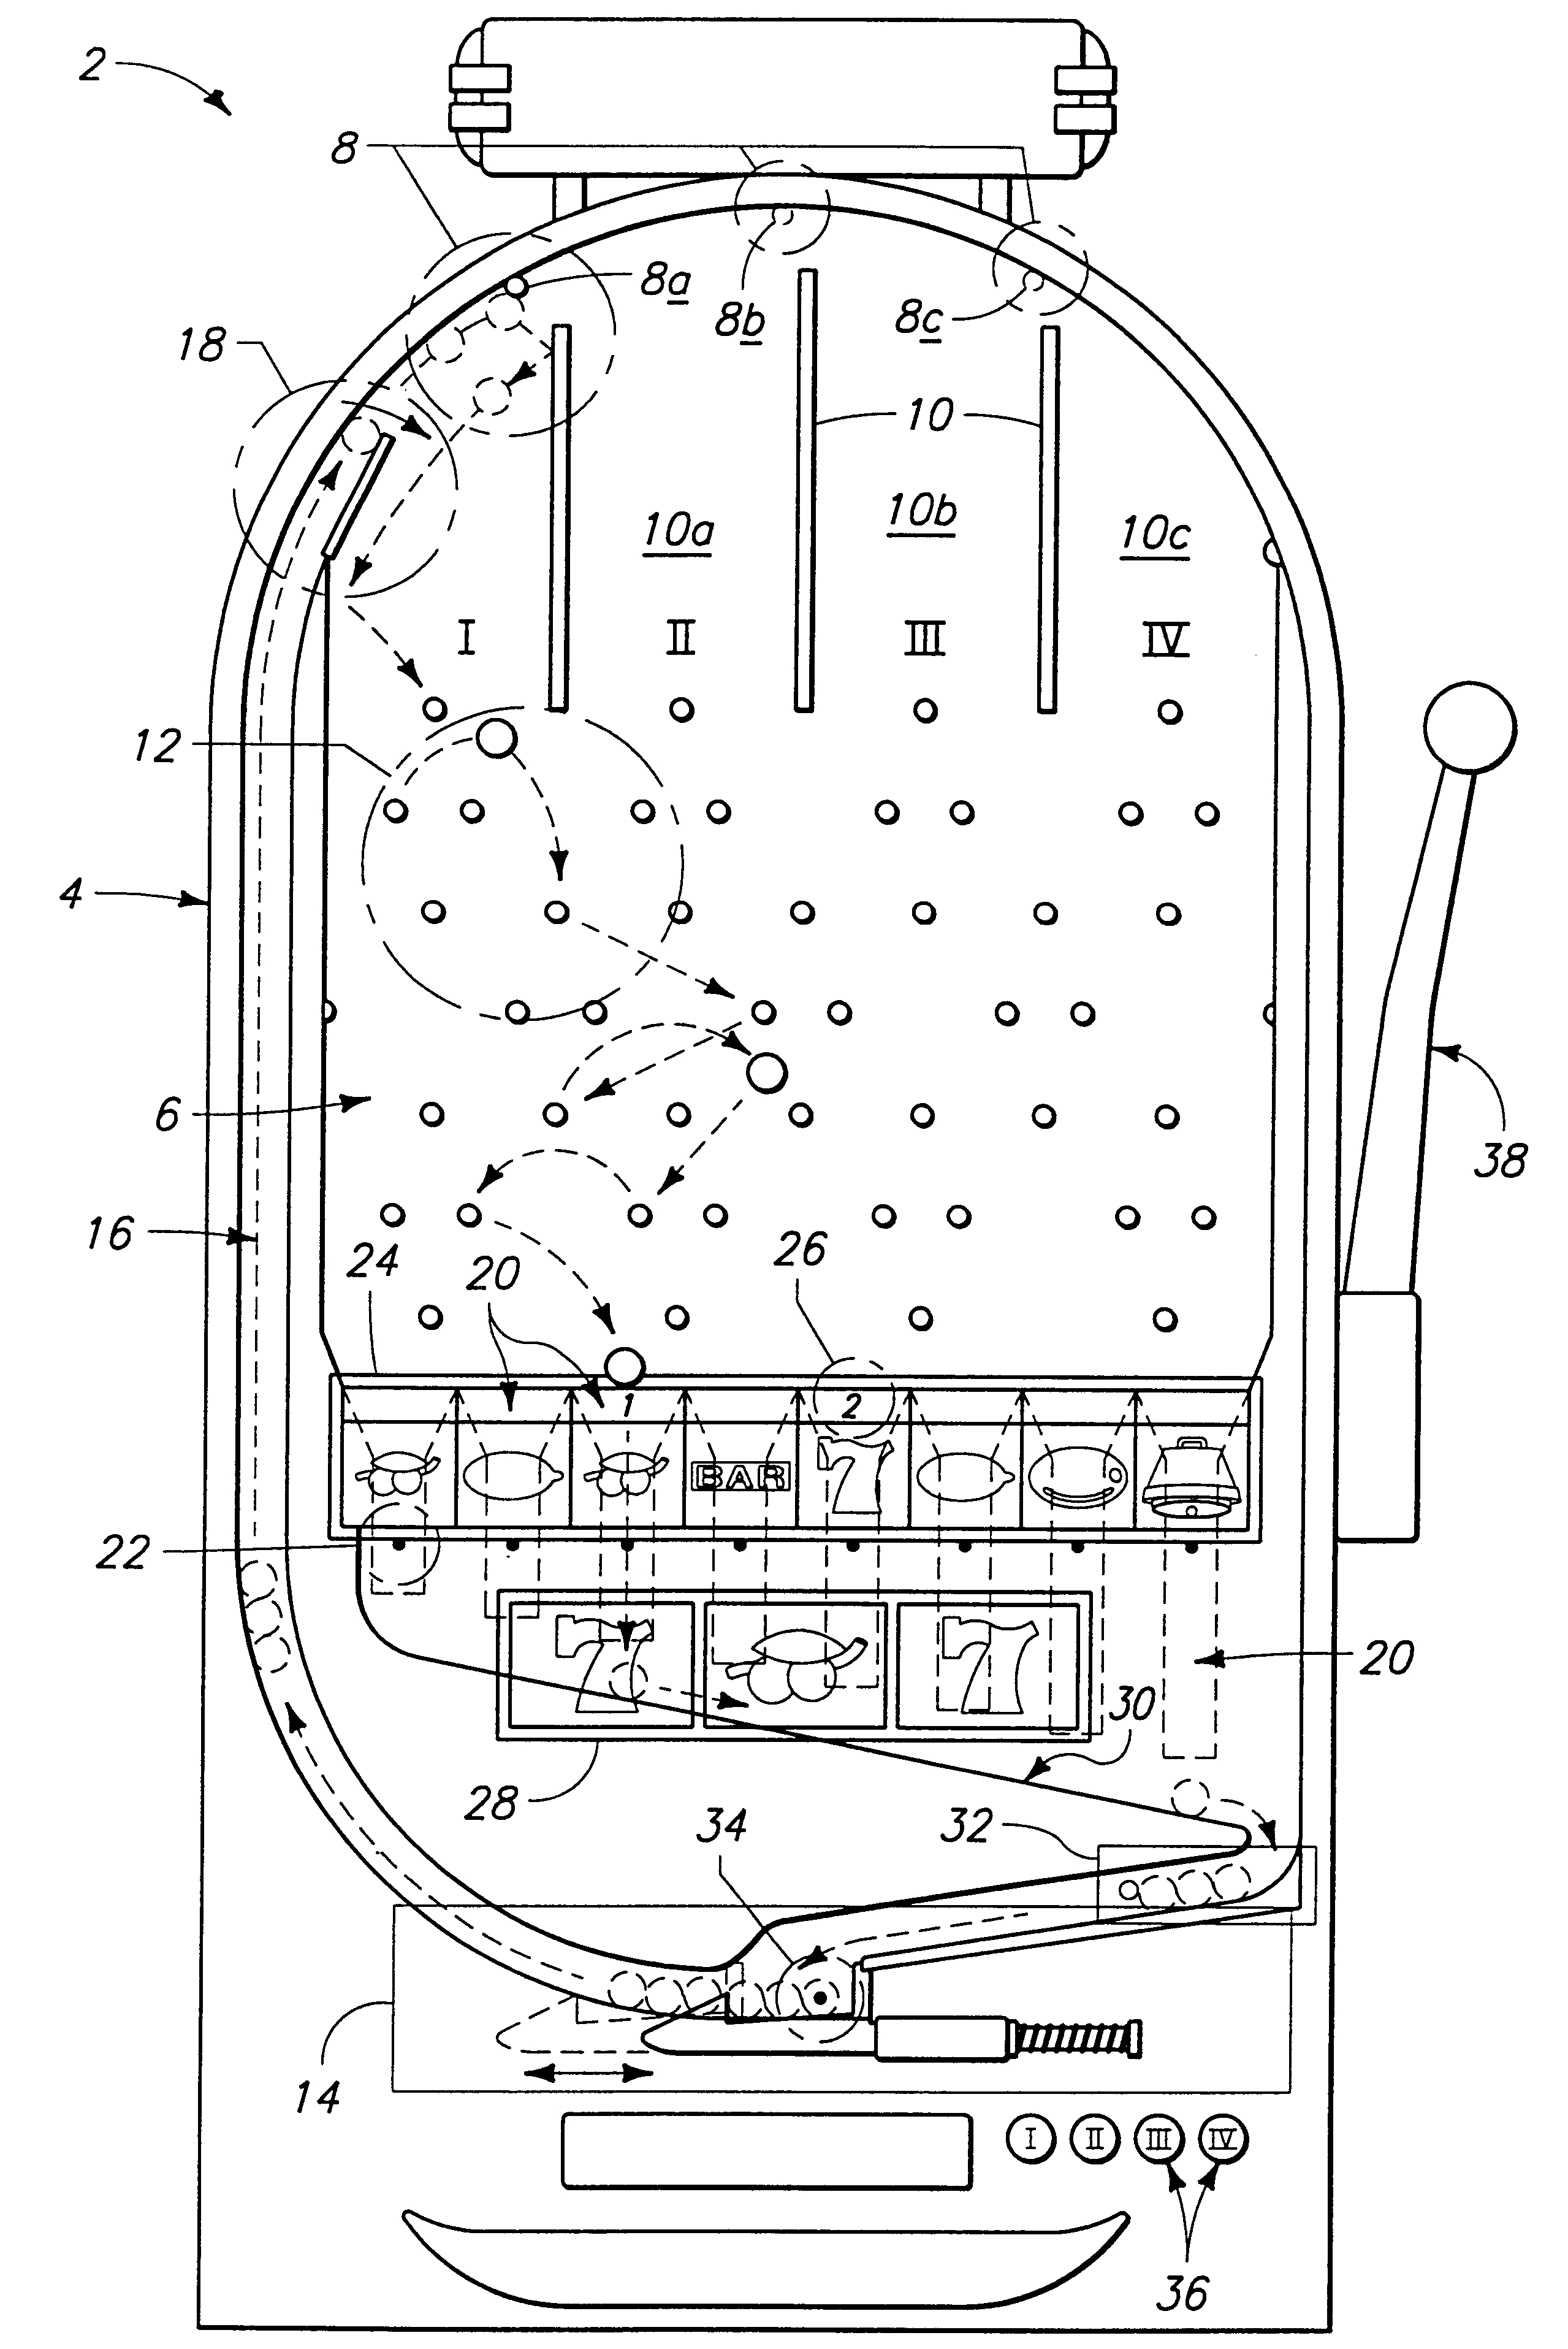
\includegraphics[height=2.25in]{pachinko}
		\end{center}
		\caption{Pachinko Machine -- A path of the ball is shown in red.}
		\label{fig:pachinko}
	\end{figure}
	\begin{center}
		\footnotesize{From
		\url{http://www.freepatentsonline.com/6619659.html}}
	\end{center}
\end{frame}
\begin{frame}{Pachinko Allocation Model}
	\begin{minipage}{0.5\linewidth}
		\begin{figure}[ht]
			\centering{
			  \includegraphics[width=2in]{pam_plate}
			}
			\caption{4-level Pachinko Model}
			\label{fig:pam_plate}
		\end{figure}
		\scriptsize{
        \begin{tabular}{llll}
            $w$ & Generated word & $M$ & \# of Documents \\
            $z_{w1}$ & Root topic  & $N$ & \# of Words\\
			$z_{w2}$ & Super topic & $S_1$ & \# of Super topics \\
			$z_{w3}$ & Sub topic & $S_2$ & \# of Sub topics
        \end{tabular}
		}
	\end{minipage}
	\begin{minipage}{0.45\linewidth}
		Generative Process
		\begin{itemize}
			\item For each topic, sample $\theta \sim Dir(\alpha)$
			\item For each word $w$ in the document,
				\begin{itemize}
					\item Sample topic path $z_w$ starting at the root topic
						node and terminating at a leaf node.  Each $z_i\sim
						mult(\theta)$.
					\item Sample word $w$ from $mult(\theta)$ of the last last
						topic along the path
				\end{itemize}
		\end{itemize}
	\end{minipage}
\end{frame}
\begin{frame}{Pachinko Allocation Model}
	\begin{figure}[ht]
		\begin{center}
			\includegraphics[width=4.25in]{pam_topics}
		\end{center}
		\caption{Discovered topics (circles), sub-topics (squares), and their dependencies
		(Figure from \cite{pachinko}).}
		\label{fig:pam_topics}
	\end{figure}
\end{frame}
\begin{frame}{Other Hierarchical Models}
	\begin{block}{Hierarchical LDA\cite{hlda}}
		\begin{itemize}
			\item Structure of topic tree is inferred using nested CRP
				\begin{itemize}
					\item \# of topics doesn't need to be specified in
				advance
				\end{itemize}
		\end{itemize}
	\end{block}
	\begin{block}{Correlated Topic Model\cite{ctm}}
		\begin{itemize}
			\item Similar to LDA, but uses Logistic
				Gaussian prior instead of Dirichlet.
				\begin{itemize}
					\item Not really hierarchical
					\item Covariance matrix models pair-wise correlation
				\end{itemize}
			\item Many parameters to estimate ($\mu,\Sigma$ for each topic)
				$\rightarrow$ slow inference
		\end{itemize}
	\end{block}
	\begin{block}{Hierarchical PAM\cite{hpam}}
		\begin{itemize}
			\item Same as PAM, except any node can 'output' a word (not just
				leaves)
			\item Structure and \# of topics pre-specified, but robust to bad
				parameterizations.
			\item Faster than HLDA, better empirical likelihood.
		\end{itemize}
	\end{block}
\end{frame}

%%%%%%%%%%%%%%%%%%%%%%%%%%%%%%%%%%%%%%%%%%%%%%%%%%%%%%%%%%%%%%%%%%%%%%%%%%%%%%%%
%\subsection{Bigram Topic Model}
\subsection{Beyond Bag of Words}
\begin{frame}{Beyond Bag of Words}
	\begin{block}{Bag of Words Assumption}
		Assumes that words order in a document is irrelevant. 
		\begin{itemize}
			\item It is mathematically convenient, but not strictly true!!!
		\end{itemize}
	\end{block}
	\begin{block}{Problem}
		Under these models all of the following sentences are equally likely:
		\begin{itemize}
			\item \textit{the department chair couches offers}
			\item \textit{the department chair offers couches}
			\item \textit{couches the chair department offers}
		\end{itemize}
	\end{block}
	\begin{block}{Solution}
		Explicitly incorporate word order into graphical model.
	\end{block}
\end{frame}
\begin{frame}{Bigram Topic Model \cite{btm}}
	\begin{minipage}{0.55\linewidth}
			\begin{center}
			  \includegraphics[width=2in]{bigram_plate}
			\end{center}
	\end{minipage}
	\begin{minipage}{0.40\linewidth}
	\begin{block}{Summary}
		\begin{itemize}
			\item Similar to LDA, except distribution of word $w_i$ is dependent on the
				topic and the previous word $w_{i-1}$.
		\end{itemize}
	\end{block}
\end{minipage}
\end{frame}
\begin{frame}{Bigram Topic Model \cite{btm}}
	\begin{minipage}{0.45\linewidth}
		\begin{center}
			\includegraphics[height=2in]{bigram_plate}
			\end{center}
		\end{minipage}
		\begin{minipage}{0.5\linewidth}
			Generative Process
			%Start with a dictionary of words, $\{w\}$, and set of topics $\{z\}$
			\begin{itemize}
				\item for each topic, word pair ($z,w$), draw a discrete distribution
					$\sigma_{zw}$ from a Dirichlet prior $\delta$\\
					%\pause
					%\textit{$\sigma_{zw}$ encodes the probability distribution of
					%the ``next word'' in a bigram, given the first word is $w$ and the topic $z$.}
					\pause
				\item for each document $d$, draw a discrete distribution
					$\theta^{(d)}$ \\
					\pause
					%\textit{$\theta^{(d)}$ encodes the probability distribution of
					%topics for the document $d$.}
					%\pause
					\item For each position $i$ in document $d$, draw: \\
						\footnotesize{a topic $z_i^{(d)}$ from Discrete( $\theta^{(d)}$
						)} \\
						\footnotesize{a word $w_i^{(d)}$ from Discrete( $\sigma_{zw}$ )}
				\end{itemize}
			\end{minipage}
\end{frame}
\begin{frame}{Bigram Topic Model}
	\begin{figure}
	\begin{minipage}{0.5\linewidth}
		\begin{center}
			LDA Topic Model
		\end{center}
		\begin{center}
			\tiny{
			\begin{tabular}{|c|c|c|c|}
				\hline
				the   &      i    &    that &  easter\\
				``number'' &     is   &   proteins & ishtar\\
				in   &   satan   &     the  &     a\\
				to   &    the     &     of  &    the\\
				espn   &   which     &    to  &   have\\
				hockey  &    and      &     i  &   with\\
				a   &     of      &    if   &   but\\
				this & metaphorical& ``number'' &english\\
				as  &     evil     &   you  &    and\\
				run   &    there    &   fact   &    is\\
				\hline
			\end{tabular}}
		\end{center}
	\end{minipage}
	\begin{minipage}{0.45\linewidth}
		\begin{center}
			Bigram Topic Model
		\end{center}
		\begin{center}
			\tiny{
			\begin{tabular}{|c|c|c|c|}
				\hline
				party  &   god   & ``number''  &    the\\
				arab &  believe  &   the    &     to\\
				power &   about   &  tower   &     a\\
				as  &  atheism  &  clock   &    and\\
				arabs &    gods   &    a     &     of\\
				political & before  &  power    &     i\\
				are   &   see & motherboard  &   is\\
				rolling & atheist &    mhz   &  ``number''\\
				london  &   most  &  socket  &     it\\
				security &  shafts &  plastic  &  that\\
				\hline
			\end{tabular}}
		\end{center}
	\end{minipage}
	\caption{Comparison of discovered topics between LDA and Bigram model (From
	\cite{btm})}
	\label{fig:bigram_compare}
\end{figure}
\end{frame}
\begin{frame}{Other N-Gram Topic Models}
	\begin{block}{Topical N-grams \cite{tng}}
		\begin{itemize}
			\item Similar to Bigram model, but introduces a latent indicator
				variable which specifies whether to generate a bigram.
				\begin{itemize}
					\item bigram generation is dependent on context
				\end{itemize}
			\item Allows meaning disambiguation
				\begin{itemize}
					\item i.e. \textit{white house} has a different meaning in the
						context of politics than it does in real estate.
				\end{itemize}
		\end{itemize}
	\end{block}
	\begin{block}{LDA Composite Model \cite{ldacol}}
		\begin{itemize}
			\item Similar to Bigram model, but overlays an HMM over the word
				sequence.
				\begin{itemize}
					\item Allows integration of syntactic models.
				\end{itemize}
		\end{itemize}
	\end{block}
\end{frame}

\begin{frame}{Topic Models: Extensions}
	\begin{center}Questions?\end{center}
\end{frame}
%%%%%%%%%%%%%%%%%%%%%%%%%%%%%%%%%%%%%%%%%%%%%%%%%%%%%%%%%%%%%%%%%%%%%%%%%%%%%%%%
\subsection{Application: Object Recognition in Images}
\begin{frame}{Application: Object Recognition in Images}
	\begin{block}{General Goal}
		Given an image, determine if it contains a particular object
	\end{block}
	\begin{block}{Approach}
		Model a database of labeled images using mixtures of topics,
		where:
		\begin{itemize}
			\item Each image is a document
			\item Quantize image feature patches into \textit{visual words}
			\item Each image class corresponds to a distribution of topics.
		\end{itemize}
		Given a new unlabled image:
		\begin{itemize}
			\item Infer distribution of topics for the image
			\item Find image class with most similar topic distribution 
		\end{itemize}
	\end{block}
\end{frame}
\newcommand{\cvprslide}[1]{
\begin{frame}{Application: Object Recognition in Images #1}
	\begin{figure}[ht]
		\begin{center}
			\includegraphics[width=3.5in]{cvpr#1}
		\end{center}
		\label{fig:cvpr#1}
	\end{figure}
	\footnotesize{Slides from \cite{feifei2007}}
\end{frame}
}
\cvprslide{1}
\cvprslide{2}
\cvprslide{3}
\cvprslide{4}
\cvprslide{5}
\cvprslide{6}
\cvprslide{7}
\cvprslide{8}
%%%%%%%%%%%%%%%%%%%%%%%%%%%%%%%%%%%%%%%%%%%%%%%%%%%%%%%%%%%%%%%%%%%%%%%%%%%%%%%%
\begin{frame}{}
	\begin{center}
		Questions?
	\end{center}
\end{frame}
		\begin{frame}
\frametitle{References}
\footnotesize{
\begin{thebibliography}{Blei et al, 2003}

\bibitem[Blei et al, 2003]{blei:jmlr03}
D. M. Blei, A. Y. Ng and M. I. Jordan.
Latent Dirichlet Allocation.
{\it JMLR}, 2003.
\bibitem[Blei, et al. 2003]{hlda}D. Blei, T. Griffiths, M. Jordan, and J. Tenenbaum. Hierarchical
	topic models and the nested Chinese restaurant process. NIPS 2003.

\bibitem[Blei and Laferty, 2006]{ctm} D. Blei and J. Laferty. Correlated Topic Models. NIPS 2006.

\bibitem[Cohn and Hofmann, 2001]{cohn:nips01} 
D. Cohn and T. Hofmann.
The missing link - a probabilistic model of document content and hypertext connectivity.
{\it NIPS}, 2001.

\bibitem[Hofmann, 1999]{hofmann:sigir99}
T. Hofmann.
Probabilistic Latent Semantic Indexing.
{\it SIGIR}, 1999.

\bibitem[Steyvers and Griffiths, 2006]{steyvers:inpress06}
M. Steyvers and T. L. Griffiths.
Probabilistic Topic Models. 
In {\it Latent Semantic Analysis: A Road to Meaning}.

\bibitem[Griffiths and Steyvers, 2004]{griffiths:pnas04}
T. L. Griffiths and M. Steyvers.
Finding Scientific Topics.
{\it PNAS}, 2004.

\bibitem[Griffiths et al, 2007]{ldacol}	
	Griffiths, T.L., Steyvers, M. and Tenenbaum, J.B.T. (2007). Topics in
	Semantic Representation. Psychological Review, 114(2), 211-244. 
	
\bibitem[McCallum and Nigam, 1998]{mccallum:aaaiws98}
A. Mccallum and K. Nigam.
A Comparison of Event Models for Naive Bayes Text Classification.
{\it AAAI-98 Workshop on Learning for Text Categorization}, 1998.

% Pachinko image
% www.freepatentsonline.com/6619659.html
\end{thebibliography}
}
\end{frame}
\begin{frame}{References (cont)}
\footnotesize{
\begin{thebibliography}{}

\bibitem[Madsen et al, 2005]{madsen:icml05}
R. Madsen, D. Kauchak and C. Elkan.
Modeling Word Burstiness using the Dirichlet Distribution.
{\it ICML}, 2005.

\bibitem[Li et al, 2006]{pachinko}
	Pachinko Allocation: DAG-Structured Mixture Models of Topic
	Correlations. W. Li and A. McCallum. \it{ICML 2006}.
\bibitem[Mimno et al, 2007]{hpam}
	Mixtures of Hierarchical Topics with Pachinko Allocation. D.
	Mimno, W. Li and A. McCallum. \it{ICML 2007}.
\bibitem[Rosen-Zvi, et al. 2004]{atm} M Rosen-Zvi, T Griffiths, M Steyvers and P Smyth. The Author-Topic Model for Authors and Documents. UAI 2004.
\bibitem[Wallach, 2006]{btm} H. Wallach. Topic modeling: beyond bag-of-words. ICML 2006.
\bibitem[Wang, et al. 2007]{tng} X. Wang, A. McCallum and X. Wei. Topical N-grams: Phrase and Topic
	Discovery, with an Application to Information Retrieval. ICDM 2007
\bibitem[Huang and Malisiewicz]{ctmfigure}	
	J. Huang and T.Malisiewicz. 
	Correlated Topic Model Details. 
	\url{http://www.cs.cmu.edu/~tmalisie/sword_allocation/ctm.pdf}
\bibitem[CVPR 2007 Short Course on Object Recognition]{feifei2007}
	L. Fei Fei. Bag of words models. CVPR 2007 Short Course. Presentation
	Slides.  \url{http://vision.cs.princeton.edu/documents/CVPR2007_tutorial_bag_of_words.ppt}

\end{thebibliography}
}
\end{frame}

\end{document}
